\section{Generic Programming}
\vspace{-4pt}
\begin{sectionbox}
\subsection{Type-Genericity}
\textbf{Class Templates}\smallskip
\begin{itemize}
    \item Given an implementation, e.g. class \lstinline{BST}, for a single, specific element type, e.g. \lstinline{int}, replace each occurence of the element type with a placeholder \lstinline{T}
    \item Prepend the class with \lstinline{template<typename T>}.
    \item \lstinline{Node<type>} creates a type-specific instance of \lstinline{Node}, using the substitution \lstinline{T=type}. Therefore, \lstinline{Node<T>} is sometimes called a \textbf{type constructor}.
    \item The compiler generates the code of each instantiated class for us.
\end{itemize}
\textbf{Function Templates}\smallskip
\begin{itemize}
    \item Given an implementation, e.g. \lstinline{BST::insert()}, for a single, specific element type, e.g. \lstinline{int}, replace each occurence of the element type with a placeholder \lstinline{T}.
    \item Prepend the function with \lstinline{template<typename T>}.
\end{itemize}
\textbf{Type Inference}\smallskip
Generally, the types must be explicitly specified upon instantiation (e.g. \lstinline{Node<int>}); with C++17, type inference improved.
\textbf{Type Checking}\smallskip
Commonly, one has to enforce certain properties of a generic type, typical examples are: 
Default-Constructable, Iterable, Copyable, Comparable
\end{sectionbox}
\vspace{-4pt}
\begin{lstlisting}[language=C++]
template <typename T>
class Node { 
    T key;
    Node* left, right;
public:
Node(T t, Node* l, Node* r): key(t), left(l), right(r) {}
bool contains(T search_key) const {
    if (search_key < key) {
        return left->contains(search_key); 
    }
    else {...}
}
bool insert(T insert_key) { ... }

T max() const { ...}
...
};  
\end{lstlisting}
\begin{lstlisting}[language=C++]
// For free functions
template <typename T> 
void swap(T& x, T& y) {
    T temp = x; x = y;
    y = temp;
}

// For free functions
template <typename Iter>
bool is_sorted(Iter begin, Iter end) {
    ...
}

// For operators
template <typename T>
ostream& operator<<(ostream& out, const Node<T> root) {
    ...
}

// For member functions
template <typename E>
class vector {
    ...
    
    template <typename C>
    void push_back_all(const C& other) {...} 
};
\end{lstlisting}
\vspace{-4pt}
\begin{sectionbox}
\subsection{Algorithmic Genericity}\smallskip
\begin{itemize}
    \item \textbf{Higher-Order functions}: If a type-generic function takes a callable object as an argument, it is called a higher order function; these functions are \textbf{parametric in their functionality}.
    \item \textbf{Functors}: Callable Objects with a state
\end{itemize}

\end{sectionbox}
\begin{lstlisting}[language=C++]
// generic filter function
template <typename C, typename P>
C filter(const C& src_data, P pred) {
    C data;
    for (const auto& e : src_data)
        if (pred(e)) data.push_back(e); 
    return data;
}

// stateless predicate as function
bool is_nonneg(int i) {
    return 0 <= i; // lower bound fixed
}

// stateful predicate as functor
template <typename T> struct At_least {
    T min;

    At_least(T m): min(m) {};

    bool operator()(T i) const {
        return min <= i;
    } 
};

int main () {

    std::vector<int> data = {-1,0,1,2,-2,4,5,-3};
    sel1 = filter(data, is_nonneg); // {0,1,2,4,5}
    sel2 = filter(data, At_least(-1)); // = {-1,0,1,2,4,5}
    sel3 = filter(data, At_least(4)); // = {4,5}
}
\end{lstlisting}

\begin{sectionbox}
\subsection{Lambda Expressions}\smallskip
anonymous functions - function object - function literal\par
In C++: just syntactic sugar, compiler generates a suitable functor

\textbf{General form:}
\begin{center} 
    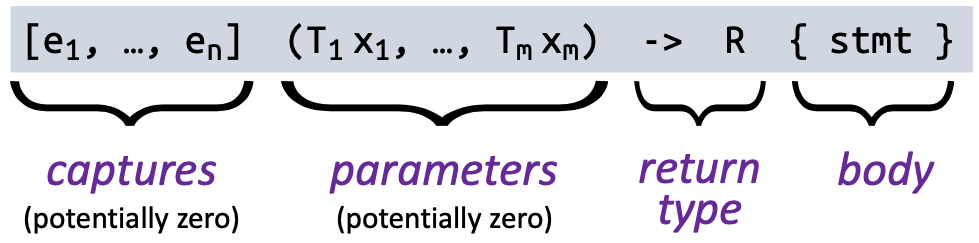
\includegraphics[width=\columnwidth]{img/Lambda.png}
    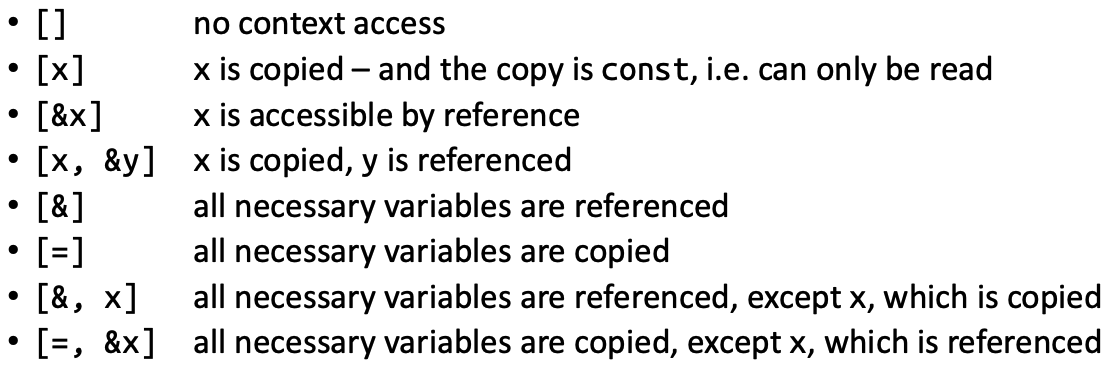
\includegraphics[width=\columnwidth]{img/LambdaCaptures.png}
\end{center}
\end{sectionbox}
